%
% projektion.tex
%
% (c) 2018 Prof Dr Andreas Müller, Hochschule Rapperswil
%
\documentclass[tikz]{standalone}
\usepackage{times}
\usepackage{amsmath}
\usepackage{txfonts}
\usepackage[utf8]{inputenc}
\usepackage{graphics}
\usetikzlibrary{arrows,intersections,math}
\begin{document}

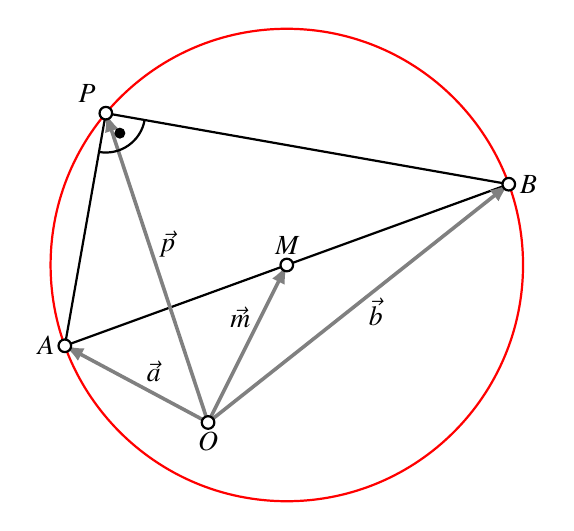
\begin{tikzpicture}[>=latex,thick]

\def\punkt#1{
	\fill[color=white] #1 circle[radius=0.08];
	\draw #1 circle[radius=0.08];
}

\def\r{3}
\def\a{20}
\def\b{140}

\def\A{({\r*cos(\a+180)},{\r*sin(\a+180)})}
\def\B{({\r*cos(\a)},{\r*sin(\a)})}
\def\C{({\r*cos(\b)},{\r*sin(\b)})}
\def\O{(-1,-2)}
\def\M{(0,0)}

\draw \A--\B--\C--cycle;
\draw[color=red] (0,0) circle[radius=\r];

\node at \A [left] {$A$};
\node at \B [right] {$B$};
\node at \C [above left] {$P$};
\node at \M [above] {$M$};

\node at \O [below] {$O$};

\draw[->,line width=1.3pt,color=gray] \O--\A;
\draw[->,line width=1.3pt,color=gray] \O--\B;
\draw[->,line width=1.3pt,color=gray] \O--\C;
\draw[->,line width=1.3pt,color=gray] \O--\M;

\node at ({(-1-\r*cos(\a))/2},{(-2-\r*sin(\a))/2-0.1}) [above right] {$\vec{a}$};
\node at ({(-1+\r*cos(\a))/2},{(-2+\r*sin(\a))/2+0.2}) [below right] {$\vec{b}$};
\node at ({(-1+\r*cos(\b))/2-0.1},{(-2+\r*sin(\b))/2+0.3}) [right] {$\vec{p}$};
\node at (-0.333,-0.666) [left] {$\vec{m}$};

\draw ({\r*cos(\b) + 0.5*cos((\a+\b)/2+180)},{\r*sin(\b) + 0.5*sin((\a+\b)/2+180)})
	arc ({(\a+\b)/2+180}:{(\a+\b)/2+270}:0.5);

\fill ({\r*cos(\b) + 0.31*cos((\a+\b)/2+225)},{\r*sin(\b) + 0.31*sin((\a+\b)/2+225)})
	circle[radius=0.07];

\punkt{\A}
\punkt{\B}
\punkt{\C}
\punkt{\M}
\punkt{\O}

\end{tikzpicture}

\end{document}

